

\documentclass[conference]{IEEEtran}

\usepackage[utf8]{inputenc}
\usepackage[pdftex]{graphicx}
%\usepackage{unicode-math}
%\usepackage{mathtools}
\usepackage{amsmath}


\hyphenation{op-tical net-works semi-conduc-tor}


\begin{document}

\renewcommand{\abstractname}{Resumo}
\renewcommand{\refname}{REFERÊNCIAS}
\renewcommand{\tablename}{TABELA}


\title{Análise de Complexidade e Experimental de Algoritmos de Ordenação}


% author names and affiliations
% use a multiple column layout for up to three different
% affiliations
%\author{\IEEEauthorblockN{Bruno Santos de Lima\\Leandro Ungari Cayres}
%\IEEEauthorblockA{Faculdade de Ciências e Tecnologia\\
%Universidade Estadual Paulista\\
%Presidente Prudente, Brasil\\
%\textit{leandroungari@gmail.com}}
%}

\author{ 
 Bruno Santos de Lima\\ 
 \IEEEauthorblockA{Faculdade de Ciências e Tecnologia\\
Universidade Estadual Paulista\\
Presidente Prudente, Brasil \\
 \textit{brunoslima4@gmail.com}
} 
 \and 
 Leandro Ungari Cayres\\ 
 \IEEEauthorblockA{Faculdade de Ciências e Tecnologia\\
Universidade Estadual Paulista\\
Presidente Prudente, Brasil \\
 \textit{leandroungari@gmail.com} 
}
} 



% make the title area
\maketitle

% As a general rule, do not put math, special symbols or citations
% in the abstract
\begin{abstract}
O 

~\\Palavras-chave: ordenação, análise assintótica e análise experimental.

\end{abstract}


\IEEEpeerreviewmaketitle


\section{Introdução}

Diversas aplicações da atualidade envolvem um grande volume de dados, desde aplicações comerciais simples a grande aplicações científicas, todas estão nesse contexto. A organização estrutural de conjunto de dados, além de prover melhor usabilidade, também otimiza tempo e o consumo de recursos, tanto de processamento quanto de memória para a execução.

Neste contexto, este trabalho apresenta uma análise dos principais algoritmos de ordenação, o qual está dividido nas seguintes seções: na Seção 2, são apresentados os algoritmos de ordenação utilizados, indicando a abordagem utilizada no processo juntamente com a sua respectiva análise assintótica. Na Seção 3, são apresentados os estudos comparativos analisando a variações dos conjunto de dados de entrada e abordagens utilizadas na ordenação. Por fim, na Seção 4, são apresentadas as considerações finais do estudo.


\section{Algoritmos de Ordenação}


\subsection{Algoritmos baseados em Troca}


\subsubsection{Bubble Sort}

O presente algoritmo utilizada a abordagem de troca, através da permutação de elementos vizinhos, seguindo a ideia de densidade dos elementos, em que pode-se optar por varrer o arranjo levando o maior elemento (mais pesado) ao fim do vetor, ou conduzir o menor elemento (mais leve) ao início desse. Esse passo (uma das duas opções excludentemente) é realizado sucessivamente para os subvetores não ordenados remanescentes até que o vetor esteja ordenado como um todo.

A abordagem original prevê que todos os elementos adjacentes sejam comparados através de $n - 1$ iterações, porém é possível que o arranjo esteja ordenado sem que sejam necessárias todos esses ciclos. De modo a prevenir operações desnecessárias, algumas abordagens utilizam-se de \textit{flags} para a detecção de trocas, caso a última iteração tenha ao menos uma ocorrência, há necessidade de pelo menos mais uma iteração, em caso negativo, o processo pode ser encerrado.

\begin{figure}
  \caption{Modelo de comparação de elementos adjacentes.}
  \centering
    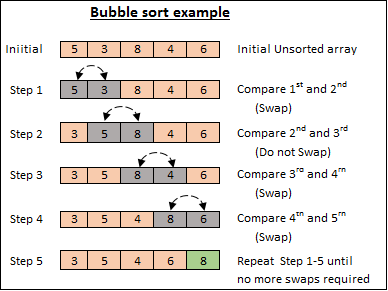
\includegraphics[width=0.4\textwidth]{images/bubble.png}
    \label{image:modelo}
\end{figure}

A Figura~\ref{image:modelo} apresenta a abordagem de ordenação utilizada pelo algoritmo referido.\\

Complexidade:
\begin{itemize}
\item \textbf{Melhor caso:} $O (n)$, para vetor crescente somente na implementação com melhoria.
\item \textbf{Caso médio:} $O (n^2)$.
\item \textbf{Pior caso:} $O (n^2)$, para vetor decrescente e aleatório.
\end{itemize}

~\\
\subsubsection{Quick Sort}

O algoritmo foi proposto por C.A.R. Hoare em 1962, tem como estratégia a divisão do arranjo original em partições a partir da determinação de um pivô. Para qualquer abordagem de escolha do pivô, em cada partição busca-se encontrar os elementos maiores que o pivô a partir do início e os menores a partir do fim do arranjo, os quais são trocados de posição aos pares, de modo a ordenar a partição, se necessário também através da quebra de subpartições.

Em relação a abordagem de escolha de pivô, há diversas técnicas que buscam explorar possíveis características dos elementos do arranjo. Dentre as principais, pode-se destacar a escolha do elemento inicial ou final do vetor, o uso de propriedades estatísticas como a média e mediana, entre outras. O principal objetivo de qualquer uma dessas estratégias é minimizar a ocorrência dos piores casos de recorrência, resultando em um comportamento assintótico quadrático.

Geralmente, os piores caso desse algoritmo consistem na escolha de pivô como elemento mínimo ou máximo, para entradas de dados crescentes e decrescentes.\\

Complexidade:
\begin{itemize}
\item \textbf{Melhor caso:} $O (nlog n)$.
\item \textbf{Caso médio:} $O (nlog n)$.
\item \textbf{Pior caso:} $O (n^2)$, em geral para o pivô mínimo e máximo.
\end{itemize}


~\\
\subsection{Algoritmos baseados em Inserção}

\subsubsection{Insertion Sort}

A estratégia de ordenação por inserção consiste em um dos métodos mais simples, sendo extremamente eficiente em conjuntos pequenos, com estratégia de percorrer o esquerdo da esquerda para a direita deixando os elementos ordenados  à esquerda. Uma situação cotidiana que aplica a abordagem referida é a inserção de cartas na mão de um jogador, seguindo a estrutura de dados deque.\\

Complexidade:
\begin{itemize}
\item \textbf{Melhor caso:} $O (n)$, para arranjo crescente.
\item \textbf{Caso médio:} $O (n^2)$.
\item \textbf{Pior caso:} $O (n^2)$.
\end{itemize}

~\\
\subsubsection{Shell Sort}

O algoritmo Shell Sort foi proposto por Donald Shell em 1959, consistindo em um dos métodos de ordenação mais eficientes dentre os modelos quadráticos, baseando-se no Insertion Sort, a partir de comparações com elementos não adjacentes, desse modo, facilitando o deslocamento dos menores elementos para o início do vetor através do uso de saltos regressivos de tamanho.

O grande diferencial desse método é a utilização dos saltos, porém não existe uma abordagem única para o cálculo do tamanho dos saltos, consistindo em um fator determinante na mensuração da complexidade assintótica. Dentre os principais modelos têm-se o $n$ primeiros múltiplos de um fator ou combinação de fatores (ex. $2^p3^q$) ou os $n$ primeiros números primos.

\begin{figure}
  \caption{Modelo de partições com elementos distantes em diferentes tamanhos.}
  \centering
    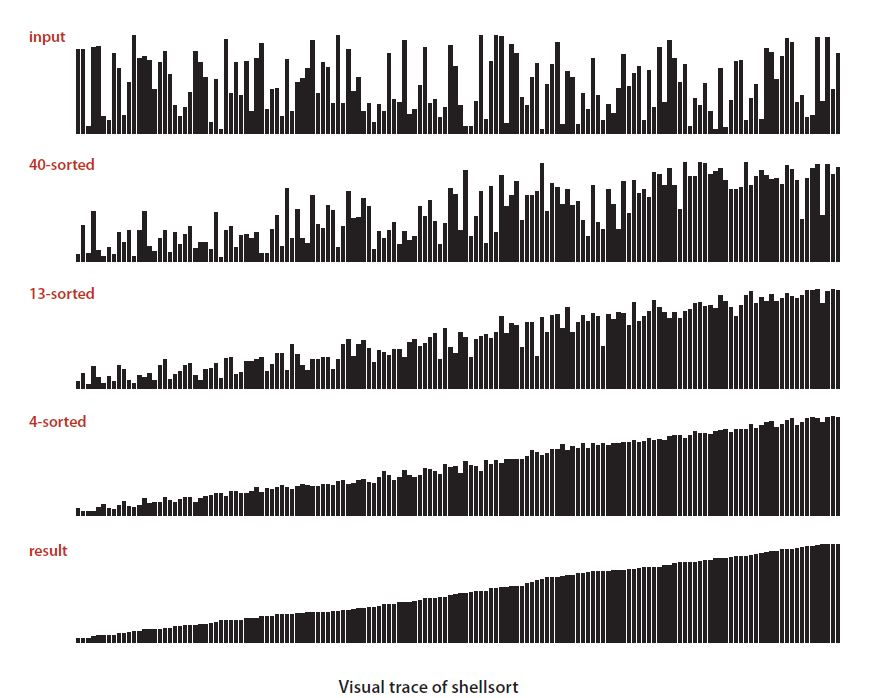
\includegraphics[width=0.4\textwidth]{images/shell.jpg}
    \label{image:shell}
\end{figure}

A Figura~\ref{image:shell} apresenta a ordenação das partições de elementos distantes, com saltos de tamanho 40, 13 e 4 respectivamente, partindo do arranjo inicial e alcançando o conjunto ordenado.\\

Complexidade:
\begin{itemize}
\item \textbf{Caso médio:} $O (n^{3/2})$
\end{itemize}
~\\
\subsection{Algoritmos baseados em Seleção}


\subsubsection{Selection Sort}

O algoritmo Selection Sort, trata-se modelo mais básico de algoritmo de ordenação, utilizada muitas em ambientes naturais e é mais intuitivo para os seres humanos, pois se utiliza da abordagem de força bruta, sem aproveitar nenhuma peculiaridade do conjunto de dados ou vantagem que possa ser tomada. Sua estratégia consiste em percorrer todo o arranjo $n$, comparando todos os elementos de forma a encontrar o menor, em seguida, o segundo menor e assim por diante, de modo a organizar todo o conjunto.

O grande destaque para esse algoritmo, dentro do contexto das abordagens quadráticas, consiste no reduzido número de trocas, que no máximo ocorre $n$ vezes.\\

Complexidade:
\begin{itemize}
\item \textbf{Caso médio:} $O (n^2)$, de modo invariante.
\end{itemize}

~\\
\subsubsection{Heap Sort}

O algoritmo Heap Sort, proposto por J.W.J. Williams em 1964, possui uma das implementações mais sofisticadas baseando-se em uma fila de prioridades, através da utilização de um vetor para a representação de uma árvore binária, caracterizando como um dos algoritmos mais estáveis de ordenação, independentemente do modelo de dados de entrada. 

\begin{figure}
  \caption{Equivalência entre a árvore e arranjo.}
  \centering
    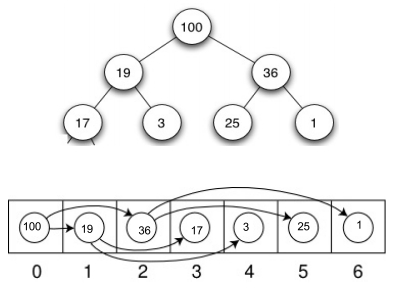
\includegraphics[width=0.4\textwidth]{images/heapsort.jpg}
    \label{image:arvore}
\end{figure}

A Figura~\ref{image:arvore} apresenta o processo de equivalência entre a estrutura de dados Heap na forma de árvore e arranjo.

O algoritmo consiste na construção de um \textit{max heap} (cuja principal propriedade consiste em que sempre o elemento raiz é maior que seus filhos, para todas as sub-árvores possíveis), em seguida, aplica-se a troca do primeiro elemento pelo último para todos os elementos do conjunto (equivalente a remover todos os elementos do arranjo), e posteriormente, rearranjar a estrutura para cada elemento, desse modo é obtido um vetor ordenado de modo crescente ao termino do processo.\\

Complexidade:
\begin{itemize}
\item \textbf{Caso médio:} $O (nlog n)$, de modo invariante.
\end{itemize}

~\\
\subsection{Algoritmos baseados em Intercalação}

\subsubsection{Merge Sort}

Este algoritmo utiliza o princípio de divisão e conquista, de modo a quebrar um problema complexo em sub-problemas, até o caso base (restante um ou dois elementos no sub-vetor), de modo que seja possível ordená-los. A partir da garantia de que todos os sub-arranjos estão ordenadas, inicia-se o processo de combinação entre eles, de modo recursivo, até alcançar o problema original, de modo ordenado.

As posições situações de ocorrência são as seguintes:
\begin{itemize}
\item em seu seu melhor caso nunca é necessário realizar trocas após comparações;
\item o caso médio ocorre quando nem sempre é necessário realizar trocas após comparações;
\item por fim, o pior caso ocorre quando sempre é necessário realizar trocas após comparações.
\end{itemize}~\\

Contudo, de modo invariável, todos os casos tem a mesma complexidade assintótica. Adicionalmente, vale-se destacar que diferentemente dos demais algoritmos que não se utilizam de memória adicional, o algoritmo Merge Sort tem complexidade espacial de tamanho $n$, que em dadas situações, deve ser levada em consideração.

\begin{figure}
  \caption{Abordagem de divisão e conquista do algoritmo.}
  \centering
    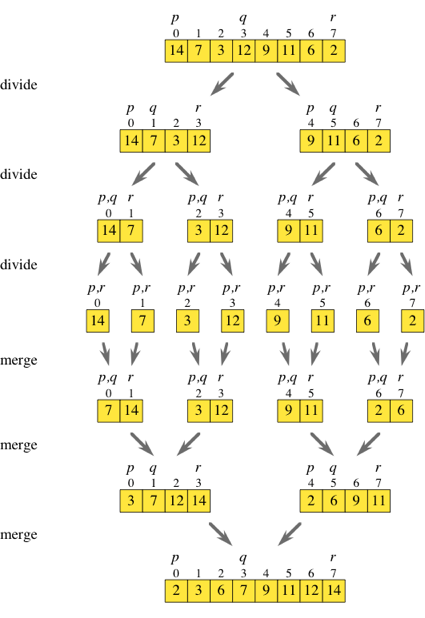
\includegraphics[width=0.4\textwidth]{images/merge.png}
    \label{image:merge}
\end{figure}

A Figura~\ref{image:merge} apresenta o processo de divisão e conquista utilizado no algoritmo.\\

Complexidade:
\begin{itemize}
\item \textbf{Caso médio:} $O (nlog n)$, de modo invariante.
\end{itemize}

~\\
%==================================
\section{Análise Experimental}

De modo a prover uma análise experimental em relação aos algoritmos, foram conduzidos estudos com diferentes tamanhos de entrada, cujas dimensões foram: 10, 100, 1 000, 10 000, 100 000 e 1 000 0000 de elementos, em que para todos os casos foram utilizados como teste um vetor crescente, decrescente e elementos dispersos pelo vetor de forma aleatória (vale ressaltar que para este último foi utilizado um arquivo que armazena os elementos, para que esta sequência aleatória seja sempre a mesma para execução em todos os algoritmos). Todos os casos foram avaliados em relação ao tempo medido em milissegundos (ms).

Para a realização da análise experimental foi utilizado um notebook com as seguintes especificações: processador Intel Core i7-7700HQ CPU @ 2.80 GHz de 4 núcleos físicos e 8 threads, com memória
caches L1 de 256 KB, L2 de 1 MB, L3 de 6 MB e memória
RAM de 8 GB DDR4.


\subsection{Modelos de entrada de dados}

\subsubsection{Entrada crescente}


\subsubsection{Entrada decrescente}


\subsubsection{Entrada aleatória}


\subsection{Comparativo de abordagem}

\subsubsection{Abordagem de inserção}


\subsubsection{Abordagem de seleção}


\subsubsection{Abordagem de troca}


\section{Considerações Finais}



\begin{thebibliography}{1}

%https://www.opentechguides.com/how-to/article/c/51/bubble-sort-c.html
%http://wiki.icmc.usp.br/images/b/b3/SCC501Cap4.pdf
%https://pt.khanacademy.org/computing/computer-science/algorithms/merge-sort/p/challenge-implement-merge-sort

\bibitem{atlas}
Programa das Nações Unidas para o Desenvolvimento (PNUD). \emph{Atlas do desenvolvimento humano do Brasil}. PNUD; 2003. Disponível em: http://www.pnud.org.br/atlas/

\bibitem{senak}
Sen AK. \emph{Desenvolvimento como liberdade}. São Paulo: Companhia das Letras; 2000.


\end{thebibliography}




% that's all folks
\end{document}


